%%%%%%%%%%%%%%%%%%%%%%%%%%%%%%%%%%%%%%%%%
% University/School Laboratory Report
% LaTeX Template
% Version 3.0 (4/2/13)
%
% This template has been downloaded from:
% http://www.LaTeXTemplates.com
%
% Original author:
% Linux and Unix Users Group at Virginia Tech Wiki 
% (https://vtluug.org/wiki/Example_LaTeX_chem_lab_report)
%
% License:
% CC BY-NC-SA 3.0 (http://creativecommons.org/licenses/by-nc-sa/3.0/)
%
%%%%%%%%%%%%%%%%%%%%%%%%%%%%%%%%%%%%%%%%%

%----------------------------------------------------------------------------------------
%	PACKAGES AND DOCUMENT CONFIGURATIONS
%----------------------------------------------------------------------------------------

\documentclass{article}

\usepackage[version=3]{mhchem} % Package for chemical equation typesetting
\usepackage{siunitx} % Provides the \SI{}{} command for typesetting SI units

\usepackage[top=1in, bottom=1in, right=1in, left=1in]{geometry}

%Add code formating
\usepackage{listings}
\lstset{tabsize=2}

\usepackage{hyperref}

\usepackage{amssymb}

\usepackage{enumerate}

\usepackage{multicol} % Multi-column support

%Add extra support for image placement
\usepackage{float}

\usepackage{mcode}

\usepackage{graphicx} % Required for the inclusion of images

\setlength\parindent{0pt} % Removes all indentation from paragraphs

\renewcommand{\labelenumi}{\alph{enumi}.} % Make numbering in the enumerate environment by letter rather than number (e.g. section 6)

%\usepackage{times} % Uncomment to use the Times New Roman font

% Setup how hyperlinks look
\usepackage{xcolor}
\hypersetup{
	colorlinks,
	linkcolor={red!50!black},
	citecolor={blue!50!black},
	urlcolor={blue!80!black},
}

%----------------------------------------------------------------------------------------
%	DOCUMENT INFORMATION
%----------------------------------------------------------------------------------------

\title{MCP3008 ADC Setup Guide} % Title

\author{Blake \textsc{Vermeer}} % Author name

\date{\today} % Date for the report

\begin{document}

\maketitle % Insert the title, author and date

\begin{center}
\begin{tabular}{l r}
Date Performed: & April 6, 2017 \\ % Date the experiment was performed
Company: & Keysight Technologies % Company
\end{tabular}
\end{center}

% If you wish to include an abstract, uncomment the lines below
% \begin{abstract}
% Abstract text
% \end{abstract}

%----------------------------------------------------------------------------------------
%	OVERVIEW
%----------------------------------------------------------------------------------------
\section{Overview}

In this tutorial you will learn about the MCP3008 ADC and how to connect and use it with the Keysight Hacking Platform development kit.


%----------------------------------------------------------------------------------------
%	What is an ADC?
%----------------------------------------------------------------------------------------
\section{What is an ADC and why do I need it?}

An Analog to Digital Converter (ADC) is a device that can measure an analog voltage and covert the measurement to a digital code that can be used by a microcontroller such as a Raspberry Pi. We need an external ADC to measure analog voltages since the Raspberry Pi does not have its own ADC built-in.

	\begin{figure}[H]
		\centering
		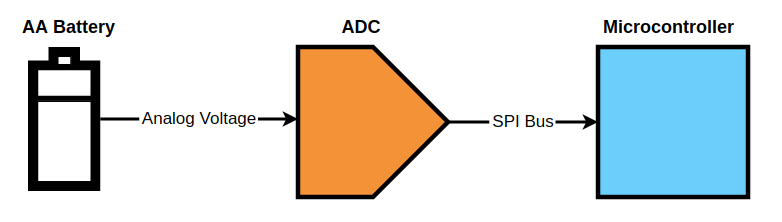
\includegraphics[width=0.75\textwidth]{pics/ADC_Dataflow.png}
		\caption{ADC Dataflow}
		\label{ADC_Dataflow}
	\end{figure}

There are several different types of ADCs from various manufacturers with varying degrees of precision. In this tutorial we will be using Microchip's MCP3008 8 channel 10-bit SPI ADC.



\section{MCP3008 Data Interface}

There are several different digital data buses that are commonly used by discrete ADCs to talk to microcontrollers (I2C, SPI, etc...). In our case the MCP3008 uses a Serial Peripheral Interface bus (SPI) for the digital data interface. An SPI bus consists of four discrete signals:

	\begin{enumerate}[1.)]
		
		\item \textbf{CLK or SCLK} - Serial clock signal generated by the master device
		
		\item \textbf{MOSI} - (Master Out Slave In) This is a serial data line for data from the master device to the slave device
		
		\item \textbf{MISO} - (Master In Slave Out) This is a serial data line for data from the slave device to the master device
		
		\item \textbf{SS or CS} - (Slave Select or Chip Select) This line is either pulled high or low (for the MCP3008 it is pulled low) by the master device to initiate communication with the slave device
		
	\end{enumerate}



%----------------------------------------------------------------------------------------
%	Connecting the MCP3008 ADC
%----------------------------------------------------------------------------------------
\section{Connecting the MCP3008 ADC to the Raspberry Pi}

Before we can connect any device we need to know the device's pinout. Figure \ref{MCP3008_pinout} is the pinout of the MCP3008 taken from its datasheet.


	\begin{figure}[H]
		\centering
		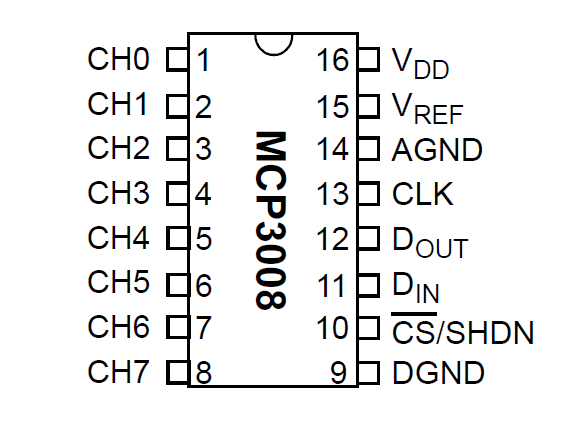
\includegraphics[width=0.5\textwidth]{pics/MCP3008_pinout.png}
		\caption{MCP3008 ADC Pinout}
		\label{MCP3008_pinout}
	\end{figure}


Notice the half-circle notch on the top of the part. This mark will help you determine where pin 1 is on the MCP3008. Figure \ref{MCP3008_pinout_labeled} labels the MCP3008's pins based on their functions.


	\begin{figure}[H]
		\centering
		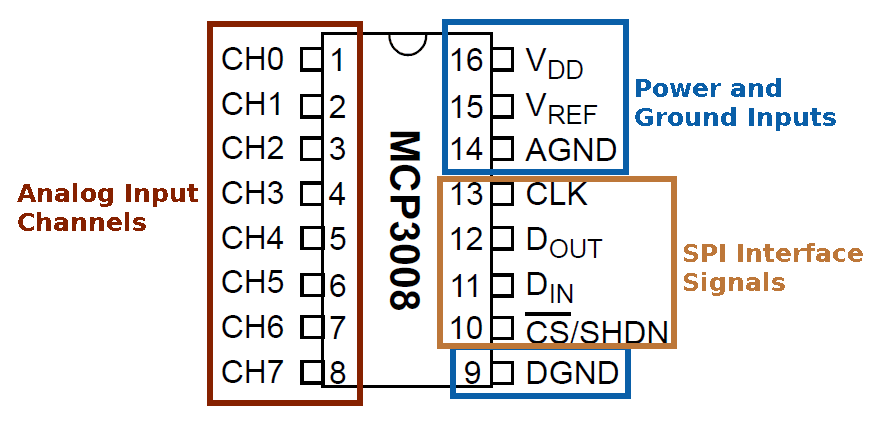
\includegraphics[width=0.95\textwidth]{pics/MCP3008_pinout_labeled.png}
		\caption{MCP3008 ADC Pinout Labeled}
		\label{MCP3008_pinout_labeled}
	\end{figure}


Now that we understand the pinout of the MCP3008, the next thing we need to figure out is which pins we need to connect to on the Raspberry Pi. The Raspberry Pi 3 has two SPI buses available on its GPIO header. If you refer to the Keysight Hacking Platform hardware guide you know that SPI bus 0 is already in use by the touchscreen. Therefore, we will use SPI bus 1 to connect to the MCP3008. The GPIO lines that are used for SPI bus 1 are show in Figure .

	\begin{figure}[H]
		\centering
		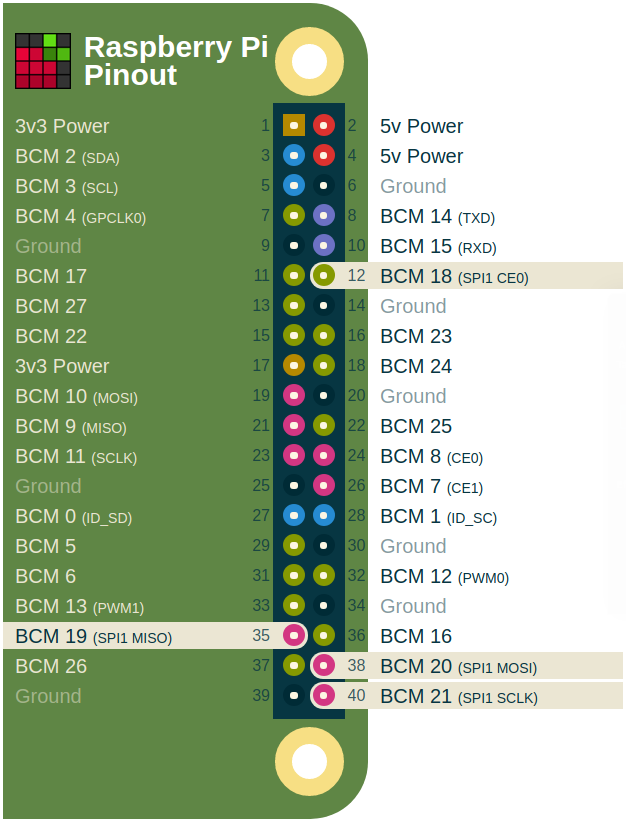
\includegraphics[width=0.5\textwidth]{pics/SPI_Bus1_CS0.png}
		\caption{Raspberry Pi 3, SPI Bus 1}
		\label{SPI_Bus1}
	\end{figure}

The last bit of information we need to know is that the Raspberry Pi 3's GPIO lines operate at 3.3V. Therefore, we will run the MCP3008 off of the 3.3V rail (the MCP3008 can run off of 3.3V or 5V). \\

After putting all this information together, we can hook the up MCP3008 to the Raspberry Pi as shown in Figure \ref{ADC_3_3_Breadboard}.

	\begin{figure}[H]
		\centering
		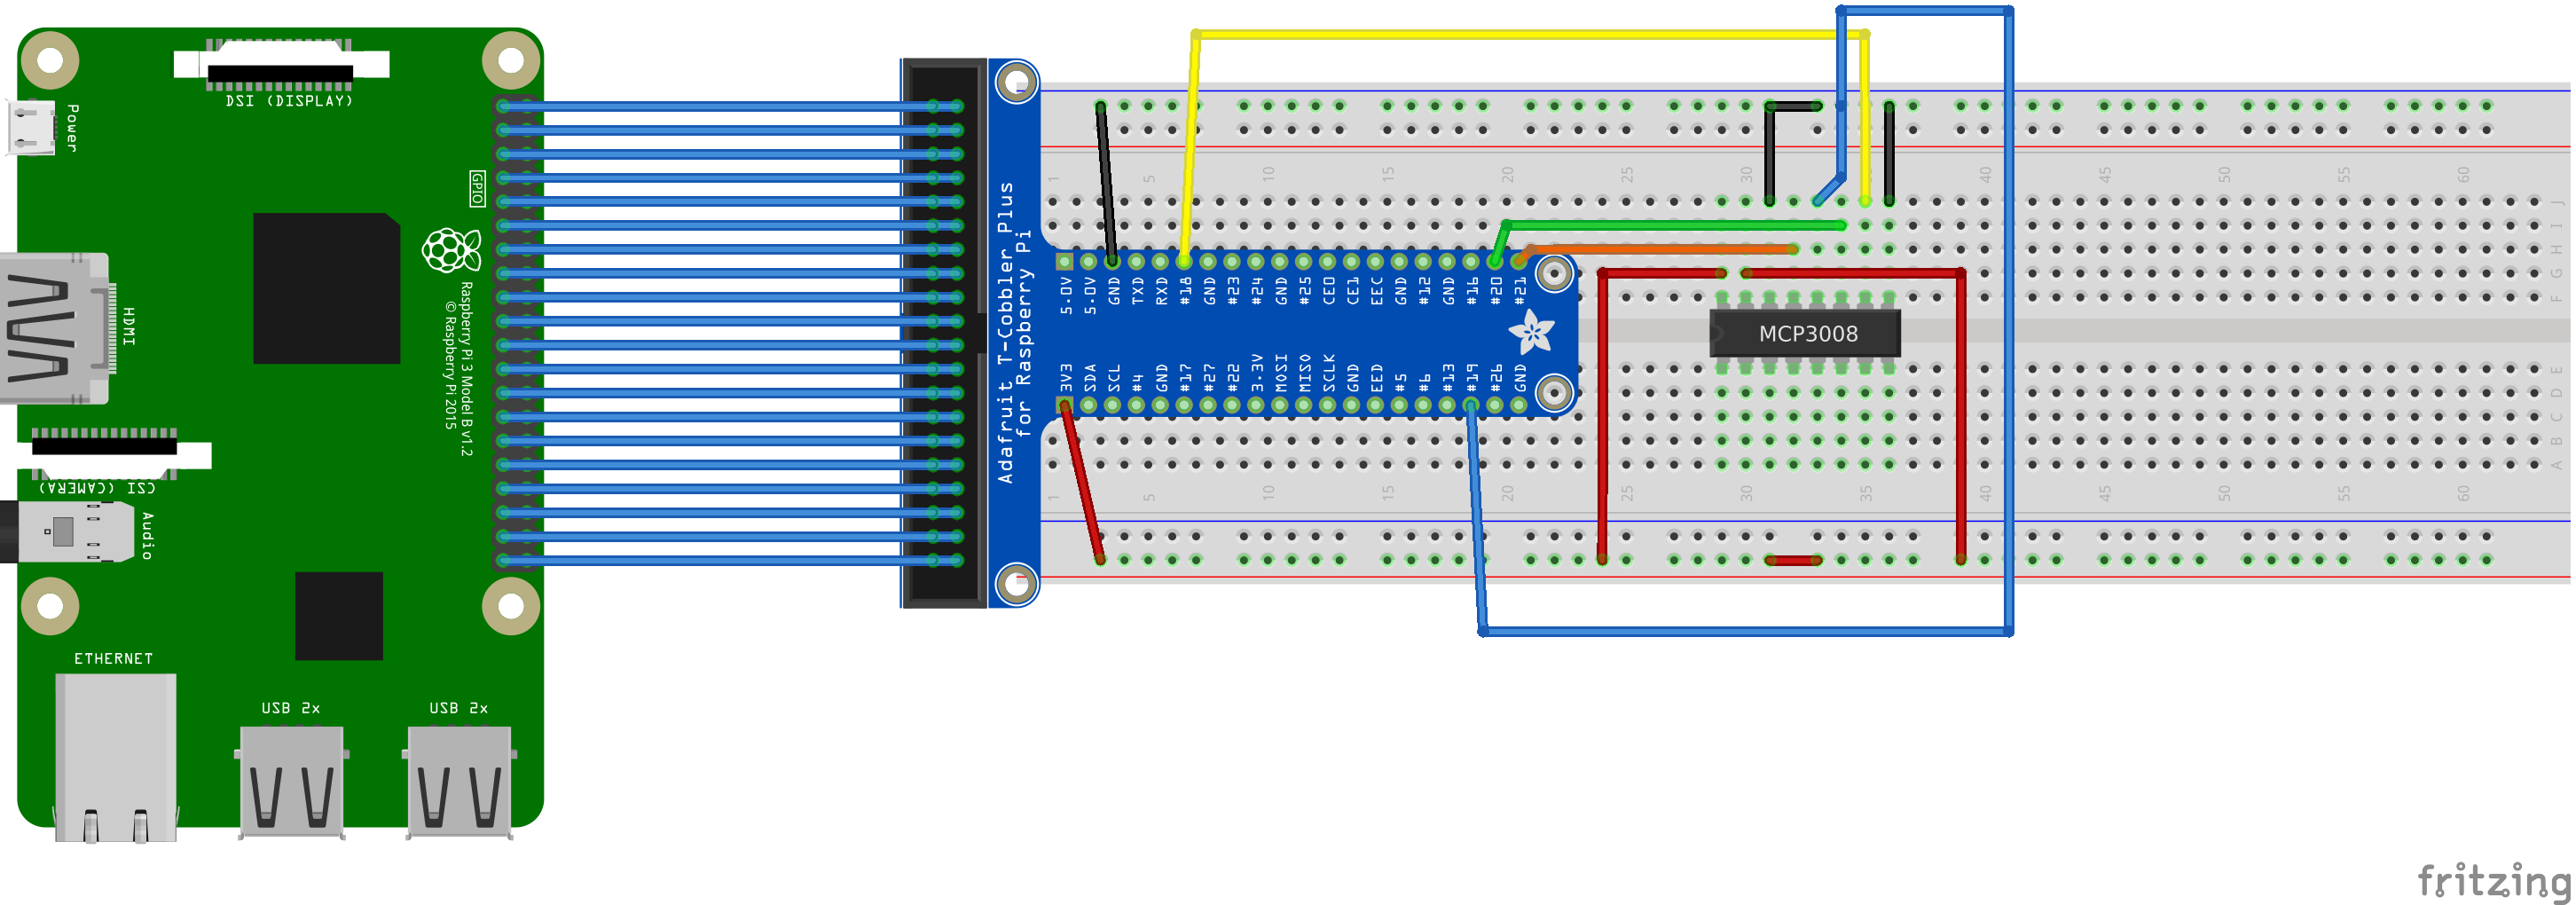
\includegraphics[width=1\textwidth]{pics/MCP3008_Breadboard_Hookup.png}
		\caption{MCP3008 ADC connection to the Raspberry Pi}
		\label{ADC_3_3_Breadboard}
	\end{figure}



%----------------------------------------------------------------------------------------
%	Converting a Measured Voltage to an ADC Code
%----------------------------------------------------------------------------------------
\section{Converting a Voltage to an ADC Code}
The MCP3008 is a 10-bit ADC. This means that the ADC will convert the voltage that it measures to a number that is between 0 and 1023. The maximum voltage the MCP3008 can measure is $V_{ref}$ which in our case is 3.3V and that can be measured is 0V. Therefore, the formula for converting the measured voltage to an ADC code is as follows:

\begin{center}
	\begin{math}
	ADC\ Code = \frac{V_{in}}{V_{ref}} * 1023 = \frac{V_{in}}{3.3V} * 1023
	\end{math}
\end{center}



%----------------------------------------------------------------------------------------
%	Notes about input voltage
%----------------------------------------------------------------------------------------
\section{Notes About Input Voltage}

Since we configured the MCP3008 to be powered from a 3.3V rail, the highest voltage we can measure is 3.3V. If you decide to use 5V devices we need to make a simple voltage divider to limit the max voltage that the ADC will see to 3.3V. This can easily be accomplished with a pair of resistors as shown in Figure \ref{Voltage_Divider}.

 
	\begin{figure}[H]
		\centering
		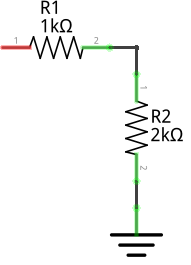
\includegraphics[width=0.25\textwidth]{pics/Voltage_Divider.png}
		\caption{2/3's Voltage Divider}
		\label{Voltage_Divider}
	\end{figure}

The 5V device will be connected to pin 1 of R1 and the ADC input channel will be connected to the junction between R1 and R2. The equation for a two resistor voltage divider is as follows:

	\begin{center}
		\begin{math}
		V_{out} = V_{in} * \frac{R2}{R1 + R2} = V_{in} * \frac{2k}{1k + 2k} = V_{in} * \frac{2}{3}
		\end{math}
	\end{center}


%----------------------------------------------------------------------------------------
%	Software to use the MCP3008
%----------------------------------------------------------------------------------------
\section{Software to use the MCP3008}

Refer to the \textbf{MCP3008\_ADC\_Example} program for a software example of how to communicate with the MCP3008. The \textbf{mcp3008Spi} class can also be used in your own project to talk to the ADC.


%----------------------------------------------------------------------------------------
%	APPENDIX
%----------------------------------------------------------------------------------------

%\newpage
%\section{Appendix}

%\begin{enumerate}

	
%	\item[1. a.)] \lstinputlisting{../MATLAB/problem_1a.m}
	

%\end{enumerate}






%----------------------------------------------------------------------------------------


\end{document}